\subsection{Metadata labels}\label{sec:appendix_meta_data}
In this section, the different types of metadata used in our evaluations are explored. 
Here the focus is on the observations related to the labels of the metadata.

\subsubsection{Metadata labels}\label{sec:appendix_meta_data}
Here are the 58 different categories, which make up all the category labels present within the dataset.

\begin{table*}[h]
	\centering
	\begin{tabular}{l|c|l|c|l|c|l|c}
		Category & Number & Category & Number & Category & Number & Category & Number \\
 		\toprule
		Udland-avis & 8855 & 26. Frederik & 484 & INFOMAKER PRINT & 5 & Thisted sport & 698\\
		Kram & 244 & Feature & 188 & Thisted-net & 3 & WEEKEND & 1493\\
		Navne & 3749 & Morsø-avis & 5959 & DF Licitation Diverse & 4 & Erhverv-avis & 7356\\
		Brønderslev-net & 3857 & Aalborg-avis & 5544 & Oplandsavisen & 6 & Biler & 13\\
		Fælles & 20204 & Mariagerfjord-avis & 7241 & Morsø Sport & 2350 & Sport-net & 3\\
		Bo Godt & 1447 & Erhvervsnavne & 39 & Debat & 10075 & Frieord & 1341\\
		RB & 3 & Hanbo-bladet & 2 & Lokalavisen & 1 & Indsigt & 984\\
		Samfund & 9 & Morsø Debat & 1375 & Sport-avis & 10941 & Kultur & 3012 \\
		53. Frederik & 203 & DF Søfart & 32 & Bagside & 1933 & Morsø-net & 1 \\
		Frederikshavn-avis & 4325 & Nordjyske Biler & 1400 & Østvendsyssel Avis & 4 & Aalborg:nu & 73\\
		Perspektiv & 613 & Brønderslev-avis & 3857 & Rebild-avis & 4415 & Brugermappe & 1\\
		Thisted-avis & 11473 & DF Motor Biler & 3 & Nyhedsmotoren-net & 3 & Morsø Ugeavis & 27\\
		Jammerbugt-avis & 3791 & MitLiv & 1519 & Newspack & 35 & DF Licitation Byggeri & 14\\
		Mariagerfjord-net & 1 & Hjørring-avis & 4235 & Friii & 2333 & Vesthimmerland-avis & 5131\\
		Plus Publicering & 3 & Nordjyske Plus & 6 & & & & \\
		\bottomrule
	\end{tabular}
	\caption{Amount of documents with each category within the Nordjyske dataset from 2017 to 2019.}
	\label{tab:category_table}
\end{table*}

\subsubsection{Author Metadata}
There are a total of $227$ authors within the dataset where each author on average have written $757$ articles from 2017 to 2019.
An interesting fact is that the median is $316$ which is much lower than the average which is visible in \autoref{fig:author_histogram}.
This shows that while most authors have written just a few hundred articles, there is a small amount of authors that have written thousands of articles, increasing the average.
The minimum number of articles that have been written by an author is $1$ and the maximum number is $9906$.
When we look at the top two most writing authors, we get these:
\begin{itemize}
	\item Ove Nørhave (9893 articles)
	\begin{itemize}
		\item A well-known journalist, who have been at Nordjyske for over 25 years.
	\end{itemize}
	\item System Administrator (9038 articles)
	\begin{itemize}
		\item We are not sure why this has been used, it could be a placeholder.
	\end{itemize}
\end{itemize}

 
\begin{figure}
	\centering
	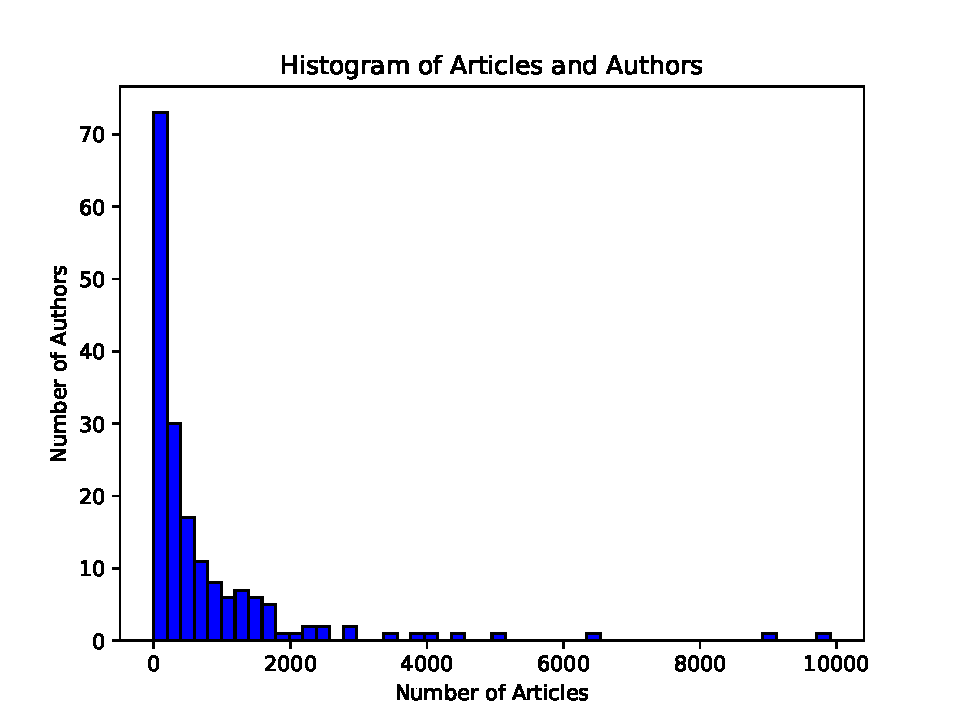
\includegraphics[width=.7\linewidth]{figures/author_hist_plot.pdf}
	\caption{A histogram over the number of articles authors have written.}
	\label{fig:author_histogram}
\end{figure}
In \autoref{fig:author_histogram}, we see that the vast majority of authors have written under $2000$ articles within the three years. 
All authors and the number of articles they have written can be seen in \autoref{tab:author_table}.

Other than the 'System Administrator' author, there are a few authors that seem different since they do not have the name of a person.
These are: 'SAXoTECH Systembruger' with 1 article, 'JSLbruger Nordjyske', 'testbruger', and 'Danske Fagmedier master' with 2 articles, and 'AAArtikler parkeret' with 51 articles.
After preprocessing, only 'AAArtikler parkeret' will not be put into the 'misc' author, since it has more than 13 articles.
From their names, they seem to be test users or authors that cover specific articles.
From looking at some articles these authors have written this seems to be the case since there are no obvious patterns in the articles written.
The name 'AAArtikler parkeret' also indicates that these articles, at least at some point, were unfinished and put under this author's name.

These articles are kept in our dataset, even though we can not be certain of who wrote them.

\begin{table*}[h]
	\caption{Number of documents written by each author in the Nordjyske dataset from 2017 to 2019.
	The highlighted authors are filtered and combined during preprocessing.}
	\label{tab:author_table}
	\centering
	\scriptsize
	\begin{tabular}{l|c|l|c|l|c|l|c}
		Author                & Number & Author                     & Number & Author                       & Number & Author                       & Number \\
		\midrule
		Ove Nørhave & 9893 & Bent Stenbakken & 646 & Katrine Schousboe & 189 & \textbf{Sarah Sandhøj} & 35 \\
		System Administrator & 9038 & Lars Hofmeister & 628 & Mathias Majlund Laursen & 178 & \textbf{Suzanne Tram} & 34 \\
		Ole Fink Mejlgaard & 6518 & Anne Helene Thomsen & 606 & Anne Brik Jensen & 177 & \textbf{Sebastian Engelberth Hansen} & 33 \\
		Peter Tordrup Larsen & 5002 & Max Melgaard & 587 & Peder Pedersen & 166 & \textbf{Anna Østergaard Bjørn} & 29 \\
		Kim Juhl Andersen & 4506 & Karen Marie Foldbjerg & 580 & Carl Åge Østergaard & 152 & \textbf{Michael Sand Andersen} & 27 \\
		Jeppe Damsgaard & 4057 & Lise Larsen & 575 & Mette Siggaard & 150 & \textbf{HANNE Lindblad Jensen} & 27 \\
		Jørn Larsen & 3863 & Asbjørn Hansen & 566 & Karen Keinicke & 150 & \textbf{Mathilde Juul Back Jensen} & 25 \\
		Jørn Eriksen & 3395 & Peter Witten & 544 & Tune Kristensen & 149 & \textbf{Allan Bauer} & 19 \\
		Anders Kjærgaard & 2960 & Allan Vinding Sørensen & 534 & Morten Brændstrup & 146 & \textbf{Linse Daugaard} & 18 \\
		Søren Beukel Bak & 2811 & Dorrit Gap Jensen & 530 & Emil Halkier & 143 & \textbf{Morten Nis Klenø} & 17 \\
		Søren Olsson & 2558 & Hans Christensen & 500 & \textbf{Britt Kristensen} & 135 & \textbf{OLE SANVIG KNUDSEN} & 16 \\
		Jens Peter Svarrer & 2480 & Lars Høj & 493 & \textbf{KAREN Marie Foldbjerg} & 132 & \textbf{Frederik Siiger} & 15 \\
		Flemming Kristensen & 2282 & Jesper Ramsing & 469 & \textbf{Claus Smidstrup} & 128 & \textbf{Kim Lesanner} & 15 \\
		Thomas Jasper & 2186 & Jens Hukiær & 464 & \textbf{Sarah Thun Madsen} & 127 & \textbf{Pia Haugaard} & 13 \\
		Bente Lembo & 2128 & Svend Ole Jensen & 447 & \textbf{Jakob Kanne Bjerregaard} & 126 & \textbf{MERETE HORN} & 12 \\
		Helle Møller Larsen & 1787 & Martin Frandsen & 437 & \textbf{Lars Teilmann} & 122 & \textbf{Regitze Ørnstrup Christensen} & 12 \\
		Claus Jensen & 1739 & Tobias Brandt & 423 & \textbf{Natasha Jahanshahi} & 117 & \textbf{Inge Steen Sørensen} & 11 \\
		Esben Heine Pedersen & 1689 & Andrea Jessen Jakobsen & 423 & \textbf{Jens Ole Pedersen} & 116 & \textbf{Anika Thorø Møller} & 11 \\
		Margit Sig & 1632 & Carsten Søgaard Jensen & 420 & \textbf{Pauline Bülow} & 116 & \textbf{Tim Søgaard} & 11 \\
		Jens Fogh-Andersen & 1614 & Morten Lind & 413 & \textbf{Christoffer Green Sørensen} & 115 & \textbf{Flemming Haslund} & 10 \\
		Ole Jensen & 1611 & Esben Agerlin Olsen & 406 & \textbf{Flemming Junker} & 103 & \textbf{Henrik Nordstrøm Mortensen} & 10 \\
		David Højmark & 1549 & Carsten Hougaard & 406 & \textbf{Niklas Grønborg} & 103 & \textbf{Emil Halkær} & 9 \\
		Niels Hansen & 1512 & Dorit Glintborg & 405 & \textbf{Sofie Møller} & 99 & \textbf{Katrine Hjulmann Nielsen} & 9 \\
		Line Lykkegaard Skou & 1504 & Karin Pedersen & 397 & \textbf{Michael Strandfelt} & 98 & \textbf{John Jensen} & 8 \\
		Lars Bang Bertelsen & 1443 & Kasper Ørkild & 393 & \textbf{Anders Sønderup} & 95 & \textbf{Jacob Eggert Kabel} & 8 \\
		Villy Dall & 1408 & Marianne Isen & 387 & \textbf{Søren Kjær} & 95 & \textbf{Søren Dietrichsen} & 7 \\
		Hans Peter Kragh & 1403 & Jakob Gammelgaard & 385 & \textbf{Lone Beck} & 92 & \textbf{Nicolai Østergaard} & 6 \\
		Claus T. Kræmmergård & 1354 & Dorte Geertsen & 383 & \textbf{Torben O. Andersen} & 91 & \textbf{Søren L. Hviid} & 6 \\
		Lars Christensen & 1293 & Torben Duch Holm & 364 & \textbf{Mikkel Færgemann Viken} & 91 & \textbf{Kathrine Lykkegaard Jeppesen} & 5 \\
		Rasmus Skovbo & 1253 & Henrik Strømgaard & 362 & \textbf{Hans Henrik Rasmussen} & 90 & \textbf{Ursula Rechnagel Taylor} & 5 \\
		Anders Abildgaard & 1229 & Lisbeth Helleskov & 361 & \textbf{Steffen Bek} & 89 & \textbf{Jens Otto Barsøe} & 4 \\
		Lasse Damsgaard & 1209 & Niels Brauer & 358 & \textbf{Simon Kjær Jensen} & 86 & \textbf{Maria Berg Badstue Pedersen} & 4 \\
		Søren Østergaard & 1207 & Jesper Poulsen & 348 & \textbf{Michael Sand} & 85 & \textbf{Jacob Andersen} & 3 \\
		Hanne Lindblad Jensen & 1191 & Lars Termansen & 328 & \textbf{Julian Drud Sørensen} & 84 & \textbf{Christian Brahe-Pedersen} & 3 \\
		Charlotte Bøje & 1117 & Mikkel Eklund & 328 & \textbf{Tina Larsen} & 82 & \textbf{Helle-Lise Ritzau Kaptain} & 3 \\
		Morten Kyndby Holm & 1102 & Susie Skov & 323 & \textbf{Nils Rasmussen} & 79 & \textbf{Jane Schmidt Klausen} & 3 \\
		Lars Aare Jensen & 1084 & Birgitte Sonne & 321 & \textbf{Katrine Hjulmann} & 73 & \textbf{Ebbe Fischer} & 3 \\
		Hanne Overbye & 1075 & Anders Andersen & 315 & \textbf{Mathias Lykke} & 72 & \textbf{Stefan Buur Hansen} & 3 \\
		Lise Stenbro & 1029 & Gunnar Onghamar & 309 & \textbf{Caspar Birk} & 71 & \textbf{Camilla Pehrson} & 2 \\
		Lone Lærke Krog & 1005 & Carl Emil Nielsen & 305 & \textbf{Anna Bech Sørensen} & 69 & \textbf{Danske Fagmedier master} & 2 \\
		Carsten Tolbøll & 1004 & Emma Toftelund Poulsen & 299 & \textbf{Fie Dømler} & 65 & \textbf{testbruger} & 2 \\
		Mette Møller & 974 & Ole Sanvig Knudsen & 287 & \textbf{Poul Christoffersen} & 65 & \textbf{Anders Fuglsang} & 2 \\
		Ida Smith & 973 & Charlotte Rørth & 276 & \textbf{Søren Skov} & 56 & \textbf{Peter Kargaard} & 2 \\
		Merete Horn & 929 & Morten Appel & 273 & \textbf{Nana Sofia Hansen} & 54 & \textbf{Morten Munk Andersen} & 2 \\
		Pernille K. Damsgaard & 922 & Kristian Gull Pedersen & 266 & \textbf{Tobias Reffstrup Rasmussen} & 53 & \textbf{JSLbruger Nordjyske} & 2 \\
		Lars Løcke & 873 & Birgitte Bové & 262 & \textbf{AAArtikler parkeret} & 51 & \textbf{Jan M. Jensen} & 1 \\
		Thomas Nielsen & 841 & Helle Madsen & 258 & \textbf{Camilla Gammelgaard Johansen} & 50 & \textbf{Tom Andersson} & 1 \\
		Jakob Frey Ahrentzen & 832 & Kasper Orkild Hansen & 255 & \textbf{Klaus Færch Gjerulff} & 49 & \textbf{Jørgen la Cour-Harbo} & 1 \\
		Lise Myrup Lassen & 793 & Emil Abkjær Kristensen & 253 & \textbf{Ida Thorsen} & 48 & \textbf{Rene Sonne} & 1 \\
		Carl Chr. Madsen & 785 & Nanna Holm Hansen & 252 & \textbf{Mathias Overgaard} & 46 & \textbf{SAXoTECH Systembruger} & 1 \\
		Inge Nørregård & 746 & Bine Martine Gori & 247 & \textbf{Kirsten Østergaard} & 45 & \textbf{Andreas K. Wielandt} & 1 \\
		Jesper Schouenborg & 724 & Heidi Majgaard B. Pedersen & 244 & \textbf{Gerda Buhl Andersen} & 44 & \textbf{Per Lyngby} & 1 \\
		Jens Sønderup & 709 & Daniel Vendner & 211 & \textbf{Pia Christensen} & 44 & \textbf{Michael F. Nørfelt} & 1 \\
		Birgit Eriksen & 700 & Ida Marie Kristensen & 204 & \textbf{Dorte Rohde} & 42 & \textbf{Simon Dinsen Hansen} & 1 \\
		Søren Wormslev & 681 & Kirsten Pilgaard & 197 & \textbf{Anna Grethe Jensen} & 41 & \textbf{Mads Skov Aagurd} & 1 \\
		Knud Labohn & 653 & Marianne Dyhrberg Cornett & 192 & \textbf{Henrik Schulz} & 38 & \textbf{Benita Dreyer-Andersen} & 1 \\
		Hans Jørgen Hansen & 646 & Susanne Justsen & 191 & \textbf{Lone Heilskov} & 37 & & \\
		\bottomrule
	\end{tabular}
\end{table*}

\subsubsection{Taxonomy}\label{subsec:appendix_taxonomy}
Taxonomy is fundamentally different from the other metadata fields, in this paper.
It is not fully observed with only roughly $25\%$ of documents having a taxonomy field.
It is hierarchical, with each taxonomy containing a sequence of sub-taxonomies, such as: 'STEDER/Danmark/Nordjylland/Aalborg'.
It is also possible for each document to have multiple taxonomy sequences.
Like with authors, we remove any sub-taxonomy that is used in less than $14$ taxonomy sequences ($0.01\%$ of the number of documents).
Out of $1135$ sub-taxonomies, $779$ are removed during this preprocessing.
A subset of the taxonomies and the number of articles they appear in can be seen in \autoref{tab:taxonomy_table}.
The taxonomy tree has the following sizes: 1, 4, 32, 90, and 69.192.
The numbers $4$ and $32$ are based on the number of unique taxonomy fields observed in the dataset.
The numbers $1$, $90$ and $69.192$ are the root, number of topics and number of words, respectively.

For the labels in \autoref{tab:taxonomy_table}, the counts show the labels' sizes.
It is worth mentioning that, while the counts of the labels are directly linked to the number of documents in the whole dataset, they are also connected to the size of the previous layer's taxonomy.
For example, the label 'Danmark' is in the layer below the 'STEDER' label, where the 26145 documents of 'Danmark' is a subset of the 29535 documents of 'STEDER'.

There is also a much larger number of 'STEDER' (places) documents compared to 'EMNER' (subjects) documents, respectively 29535 compared to 5449.
In \autoref{tab:taxonomy_table}, the first label on a lower layer that comes from 'EMNER' is 'Sport' with 408 documents.
This indicates that the subject taxonomies, in general, are much smaller in size.
The \gls{pam} will then be mostly influenced by this location information compared to actual topical labels.

The labels removed during preprocessing appear, as expected, to be places or subjects that have been written about just once or a few times.
We could have combined them into a 'misc' taxonomy as we did for the category and author metadata, but decided against it because it would just be a large collection of mostly random documents.

\begin{table*}[h]
	\caption{Number of documents written by each taxonomy in the Nordjyske dataset from 2017 to 2019.
	After sorting by the number of documents, only the first 100 and last 100 taxonomies are shown.
	The highlighted taxonomies are filtered and combined during preprocessing.}
	\label{tab:taxonomy_table}
	\centering
	\scriptsize
	\begin{tabular}{l|c|l|c|l|c|l|c}
		Taxonomy                & Number & Taxonomy                     & Number & Taxonomy                       & Number & Taxonomy                       & Number \\
		\midrule
		\emph{No taxonomy} & 103928 & Farsø & 182 & \textbf{Mallorca} & 1 & \textbf{Mali} & 1 \\
		STEDER & 29535 & Skørping & 177 & \textbf{Kloning} & 1 & \textbf{Godstransport} & 1 \\
		Danmark & 26145 & Hurup & 169 & \textbf{Hjørring revyen} & 1 & \textbf{Energiforbrug} & 1 \\
		Nordjylland & 23274 & Dronninglund & 167 & \textbf{Fredensborg} & 1 & \textbf{Gedser} & 1 \\
		EMNER & 5449 & Fjerritslev & 165 & \textbf{Iværksættere} & 1 & \textbf{Mylund} & 1 \\
		Thisted & 3592 & Aabybro & 163 & \textbf{Tall ships races} & 1 & \textbf{Bygge- og anlægsbranchen} & 1 \\
		Udland & 3390 & Frankrig & 159 & \textbf{Sproget} & 1 & \textbf{Kunstig intelligens} & 1 \\
		Aalborg & 3311 & Sverige & 158 & \textbf{Grurup} & 1 & \textbf{Nielstrup} & 1 \\
		Hjørring & 2146 & Paris & 157 & \textbf{Hørning} & 1 & \textbf{Kristiansand} & 1 \\
		Frederikshavn & 1997 & Fyn & 156 & \textbf{Hem} & 1 & \textbf{Nordborg} & 1 \\
		Mariagerfjord & 1987 & Rusland & 151 & \textbf{Floorball} & 1 & \textbf{Uggerhalne} & 1 \\
		Brønderslev & 1969 & Ulykker & 150 & \textbf{Store Brøndum} & 1 & \textbf{Barmer} & 1 \\
		Vesthimmerland & 1660 & Aarhus & 145 & \textbf{Korup} & 1 & \textbf{Narkomisbrug} & 1 \\
		Hovedstadsområdet & 1380 & Tyskland & 144 & \textbf{Fødevaresikkerhed} & 1 & \textbf{Adoption} & 1 \\
		Rebild & 1289 & Moskva & 143 & \textbf{Hammershøj} & 1 & \textbf{Fødevareindustri} & 1 \\
		Jammerbugt & 1198 & Arden & 142 & \textbf{Hjerneskade} & 1 & \textbf{Smugling} & 1 \\
		København & 1125 & Politik & 139 & \textbf{CATEGORY} & 1 & \textbf{Skikke og traditioner} & 1 \\
		Hobro & 996 & Morsø & 137 & \textbf{AaB Plus} & 1 & \textbf{Kigali} & 1 \\
		Aalborg og omegn & 833 & Berlin & 132 & \textbf{Ekstremsport} & 1 & \textbf{Holtet} & 1 \\
		Thisted og omegn & 800 & Sjælland & 131 & \textbf{Mozambique} & 1 & \textbf{Fritidshuse} & 1 \\
		Midtjylland & 783 & Løkken & 129 & \textbf{Maputo} & 1 & \textbf{Årslev} & 1 \\
		Mors & 630 & New York & 124 & \textbf{Handelsskole} & 1 & \textbf{Aalborg Håndbold} & 1 \\
		Aars & 540 & Natur & 123 & \textbf{Vendsyssel Håndbold} & 1 & \textbf{Oman} & 1 \\
		USA & 478 & Erhverv & 119 & \textbf{Biludstyr} & 1 & \textbf{Turistbranchen} & 1 \\
		Frederikshavn og omegn & 410 & Spanien & 119 & \textbf{Brandstiftelse} & 1 & \textbf{Øl} & 1 \\
		Sport & 408 & Klitmøller & 118 & \textbf{Nørre Dråby} & 1 & \textbf{Forlystelsespark} & 1 \\
		England & 381 & Aalestrup & 118 & \textbf{Stae} & 1 & \textbf{Etiopien} & 1 \\
		London & 379 & Herning & 116 & \textbf{Rebild Bakker} & 1 & \textbf{Addis Abeba} & 1 \\
		Hjørring og omegn & 369 & Stockholm & 115 & \textbf{Kampsport} & 1 & \textbf{Lystsejlads} & 1 \\
		Løgstør & 368 & Madrid & 115 & \textbf{Lynnedslag} & 1 & \textbf{Herfølge} & 1 \\
		Mariagerfjord og omegn & 364 & Jerslev & 113 & \textbf{Frederikshavn White Hawks} & 1 & \textbf{Sexchikane} & 1 \\
		Brønderslev og omegn & 360 & Nørager & 111 & \textbf{Paraguay} & 1 & \textbf{Gebyrer} & 1 \\
		Skagen & 341 & Sundhed & 105 & \textbf{Asuncion} & 1 & \textbf{Frederikssund} & 1 \\
		Sæby & 334 & Sindal & 105 & \textbf{Nordkraft} & 1 & \textbf{Gadeuorden} & 1 \\
		Vesthimmerland og omegn & 327 & Brovst & 105 & \textbf{Vendsyssel Elite Badminton} & 1 & \textbf{Mjels} & 1 \\
		Syddanmark & 301 & Trafik & 99 & \textbf{Tonga} & 1 & \textbf{Katmandu} & 1 \\
		Støvring & 300 & Blokhus & 95 & \textbf{Efteruddannelse} & 1 & \textbf{Militærøvelser} & 1 \\
		Hadsund & 277 & Lønstrup & 92 & \textbf{Vin} & 1 & \textbf{Fakse} & 1 \\
		Hanstholm & 276 & Uddannelse & 91 & \textbf{Årup} & 1 & \textbf{Kulturpolitik} & 1 \\
		Kultur & 246 & Pandrup & 88 & \textbf{Fiskeripolitik} & 1 & \textbf{Skræm} & 1 \\
		Rebild og omegn & 245 & Vrå & 88 & \textbf{Gudumlund} & 1 & \textbf{Taiwan} & 1 \\
		Washington & 242 & Vorupør & 86 & \textbf{Myrhøj} & 1 & \textbf{Taipei} & 1 \\
		Jammerbugt og omegn & 229 & Øster Hurup & 85 & \textbf{Ejerslev Lyng} & 1 & \textbf{Økonomisk kriminalitet} & 1 \\
		Nørresundby & 223 & Hvalpsund & 82 & \textbf{La Paz} & 1 & \textbf{Udviklingsbistand} & 1 \\
		Mariager & 214 & Odense & 82 & \textbf{Byplanlægning} & 1 & \textbf{Kollerup} & 1 \\
		Belgien & 207 & Aså & 80 & \textbf{Ajstrup} & 1 & \textbf{Askildrup} & 1 \\
		Bruxelles & 207 & Norge & 79 & \textbf{Guatemala} & 1 & \textbf{Helsinge} & 1 \\
		Hirtshals & 197 & INDHOLDSTYPER & 79 & \textbf{Vedsted} & 1 & \textbf{Albanien} & 1 \\
		Kriminalitet & 192 & Videnskab & 78 & \textbf{Yemen} & 1 & \textbf{Tirana} & 1 \\
		Hjallerup & 190 & Israel & 78 & \textbf{Skovsted} & 1 & \textbf{Jern \& maskinindustrien} & 1 \\
		\bottomrule
	\end{tabular}
\end{table*}


Statistics over the three metadata types, before and after preprocessing, can be seen in \autoref{tab:meta_prepro_stats}.

\begin{table}
	\caption{Statistics over documents associated with metadata values, before and after preprocessing.}
	\label{tab:meta_prepro_stats}
	\centering
	\begin{tabular}{l | c | c | c | c | c}
		Metadata & Min & Max & Mean & Median & Std. \\
		\midrule
		Author & 1 & 9893 & 612.6 & 191 & 1219.7 \\
		Author (preprocessed) & 15 & 9893 & 751.7 & 323 & 1311.9 \\
		Category & 1 & 20204 & 2397.6 & 548 & 3812.1 \\
		Category (preprocessed) & 188 & 20204 & 4090.0 & 2681 & 4227.3 \\
		Taxonomy & 1 & 29535 & 123.0 & 6 & 1385.9 \\
		Taxonomy (preprocessed) & 14 & 29535 & 1598.9 & 118.5 & 9298.4 \\
	\end{tabular}
\end{table}
